\newpage{\ } 
\thispagestyle{empty} 

\chapter{Materiales y Metodolog\'ia}
\lhead{Capítulo 4. \emph{Materiales y Metodolog\'ia}} % This is for the header on each page - perhaps a shortened title
En este cap\'itulo se describir\'an los materiales a utilizar en la elaboraci\'on de la metodolog\'ia, como tambi\'en aquellos a utilizar en las diversas pruebas y validaciones. El apartado nos permitir\'a conocer diversas caracter\'isticas que presentan las im\'agenes satelitales a ser empleados en el estudio, el cual poseen mucha relevancia debido a que constituyen variables determinantes en la elaboraci\'on de constantes al flujo de procesos.\\~\\
La metodolog\'ia nos presentara las diferentes procesos o m\'odulos necesarios, para el c\'alculo de p\'erdida de carbono, en un marco general como tambi\'en en detalles.
\section{Materiales}
\subsection{Im\'agenes satelitales}
A partir de los conceptos anteriores, acerca de las im\'agenes sat\'elitales, se describir\'an los diferentes tipos por ser utilizados en el proyecto, de manera a brindar las caracter\'isticas relevantes para su elecci\'on. 
\subsubsection{Landsat}
Landsat representa la colecci\'on m\'as larga y continua en el mundo de im\'agenes satelitales con resoluciones moderadas. Cuatro d\'ecadas de im\'agenes proporciona un recurso \'unico para personas que trabajan en la agricultura, geologí\'ia, silvicultura, ordenaci\'on territorial, educaci\'on, cartograf\'ia e investigaci\'on del cambio global, como tambi\'en en respuesta de emergencias y operaciones de socorro\cite{landsatNasa}.\\~\\
Las im\'agenes est\'an disponibles desde 1972 generados por una serie de 6 sat\'elites landsat. Estos sat\'elites han sido un componente importante del Programa de Observaci\'on de la tierra perteneciente a la NASA, con tres sensores primarios evolucionando a lo largo de treinta años: MSS (Multi-spectral Scanner), TM (Thematic Mapper), y ETM+ (Enhanced Thematic Mapper Plus). 
El 11 de febrero del 2013 fue lanzado el Lansadt 8 correspondiendo al futuro de los sat\'elites landsat con dos nuevo sensores, Operational Land Imager (OLI) y el Thermal Infrared Sensor (TIRS).


\begin{table}[htbp]
	\centering
	\caption{My caption}
	\label{my-label}
	\begin{tabular}{|c|c|c|c|c|c|}
		\hline
		\multirow{2}{*}{\textbf{Landsat}} & \multicolumn{5}{c|}{\textbf{Resoluciones}}                                                             \\ \cline{2-6} 
		& \textbf{Espacial} & \textbf{Espectral} & \textbf{Radiom\'etrica} & \textbf{Temporal} & \textbf{Sensor} \\ \hline
		1                                 & 79x79 m2          & 5 bandas           & 6 bits                  & 18 dias           & MSS             \\ \hline
		2                                 & 79x79 m2          & 5 bandas           & 6 bits                  & 18 dias           & MSS             \\ \hline
		3                                 & 79x79 m2          & 5 bandas           & 6 bits                  & 18 dias           & MSS             \\ \hline
		4                                 & 30x30 m2          & 7 bandas           & 8 bits                  & 16 dias           & TM              \\ \hline
		5                                 & 30x30 m2          & 7 bandas           & 8 bits                  & 16 dias           & TM              \\ \hline
		6                                 & 30x30 m2          & 8 bandas           & 8 bits                  & 16 dias           & ETM+            \\ \hline
		7                                 & 30x30 m2          & 8 bandas           & 8 bits                  & 16 dias           & ETM+            \\ \hline
		8                                 & 30x30 m2          & 9 bandas           & 12 bits                 & 16 dias           & OLI/TIRS        \\ \hline
	\end{tabular}
	\caption{Resoluciones de los sat\'elites Landsat}
\end{table}
El Servicio Geol\'ogico de los Estados Unidos (USGS) es una agencia cientifica de los Estados Unidos, el cual proveen un producto llamado L1T (Level 1 Terrain Corrected) que implica las im\'agenes Landsat con datos pre-procesados para una precisión radiom\'etrica sistem\'atica y precisi\'on geom\'etrica mediante la incorporaci\'on de puntos de control en tierra. Estos productos est\'an en la Web de forma gratuita\cite{landsatNasa}.

\subsubsection{Vegetation Continuous Fields}
Las im\'agenes VCF (Vegetation Continuous Fields) contiene estimaciones proporcionales para los tipos de cobertura vegetal: vegetaci\'on le\~{n}osa, vegetaci\'on herb\'acea y suelo desnudo. El producto se deriva de las siete bandas del sensor MODerate-resolution Imaging Spectroradiometer (MODIS) a bordo del sat\'elite Terra, perteneciente a la NASA. El esquema de clasificaci\'on continuo del VCF puede representa \'areas terrestres heterog\'eneas mejor que los esquemas tradicionales de clasificaci\'on discreta. Mientras que los sistemas de clasificaci\'on tradicionales indican donde se concentran los tipos de cobertura del suelo, este producto VCF es magnifico para mostrar cuanto de cobertura forestal o pradera existe en cualquier parte de la tierra. Posee un resoluci\'on espacial de 250x250 metros cuadrados y la colecci\'on de im\'agenes se encuentra disponible gratuitamente en la Web\cite{gl2015Uni}.
\begin{table}[htbp]\centering
\begin{tabular}{|c|c|}
	\hline \textbf{Valor Digital} & \textbf{Representaci\'on} \\ 
	\hline 0-100 & Porcentaje de \'area vegetal \\ 
	\hline 200 & Agua \\ 
	\hline 253 & Nulo \\ 
	\hline 
\end{tabular} 
\caption{Representaci\'on del valor digital en la imagen VCF}
\end{table}

\subsubsection{Paraguay Forest Change Product}
Este producto muestra donde ocurri\'o la deforestaci\'on en Paraguay durante 1990-2000, elaborados a partir de las im\'agenes Landsat TM y ETM+. Se identificaron seis clases como bosque atl\'antico, Chaco bosques, el agua, no forestales y la deforestaci\'on. El producto puede ser utilizado como un ejemplo para evaluar cuantitativamente el cambio de cobertura terrestre, tambien el de ayudar a determinar el proceso y el patr\'on de cambio en la cubierta forestal. La imagen se encuentra disponible gratuitamente en la Web\cite{gl2015Uni}.
\begin{table}[htbp]\centering
\begin{tabular}{|c|c|c|}
	\hline \textbf{Valor digital} &\textbf{ Representaci\'on} & \textbf{Color sugerido} \\ 
	\hline 1 & Bosque Atl\'antico & Verde \\ 
	\hline 2 & Bosque Chaque\~{n}o & Verde Claro \\ 
	\hline 3 & No Bosque & Agua \\ 
	\hline 4 & Agua & Azul \\ 
	\hline 5 & P\'erdida Bosque Atl\'antico & Rojo \\ 
	\hline 6 & P\'erdida Bosque Chaque\~{n}o & Purpura Claro \\ 
	\hline 
\end{tabular} 
\caption{Representaci\'on del valor digital en la imagen PFCP.}
\end{table}


\subsection{Software}
Se utilizaran dos sistemas de informaci\'on geogr\'afica que nos permitir\'an manipular los raster como tambi\'en dise\~{n}ar e implementar los algoritmos a ser utilizados en la metodolog\'ia propuesta.
\subsubsection{GRASS}
GRASS es un software SIG  bajo licencia GPL (software libre). Puede soportar informaci\'on tanto raster como vectorial y posee herramientas de procesado digital de im\'agenes. Esta disponibles principalmente para plataformas Linux.
\subsubsection{Quantum GIS}
Quantum GIS es un SIG de c\'odigo libre para plataformas GNU/Linux, Unix, Mac OS, Microsoft Windows y Android. La principal diferencia con el GRASS es la interfaz amigable con que cuenta y la facilidad de integraci\'on con nuevas funciones espaciales desarrollados por los usuarios, esto es posible debido a que la aplicaci\'on posee un soporte muy estable para lenguajes amplios en el manejo de datos espaciales, siendo C++ y python.
\section{Metodolog\'ia}
Con los conceptos y materiales planteados en anteriores apartados, se pretende establecer una flujo de procesos o m\'odulos necesarios para el logro de los objetivos en la investigaci\'on. Se busca que los algoritmos a implementar sean ligeros en cada proceso, de manera a evitar c\'alculos complejos y excesivas supervisiones, para ello es necesario determinar comportamientos estad\'isticos de la cobertura vegetal, representados en las im\'agenes satelitales, que actuaran como variables constantes en cada proceso. 

\begin{figure}[!hbtp]
	\centering
	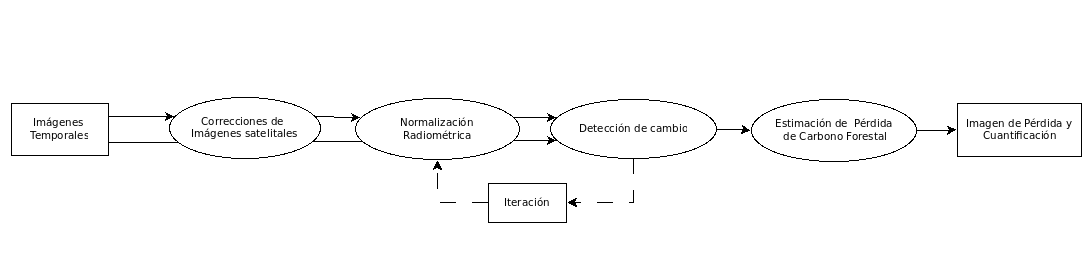
\includegraphics[width=1.0	\textwidth]{./Figures/cap4/metodologia.png}
	\caption{Diagrama de flujo. Metodolog\'ia propuesta}
	\label{fig:metodologiapc}
\end{figure}


%\begin{figure}[H]
%\centering
%\subfigure[Imagen de retina.]{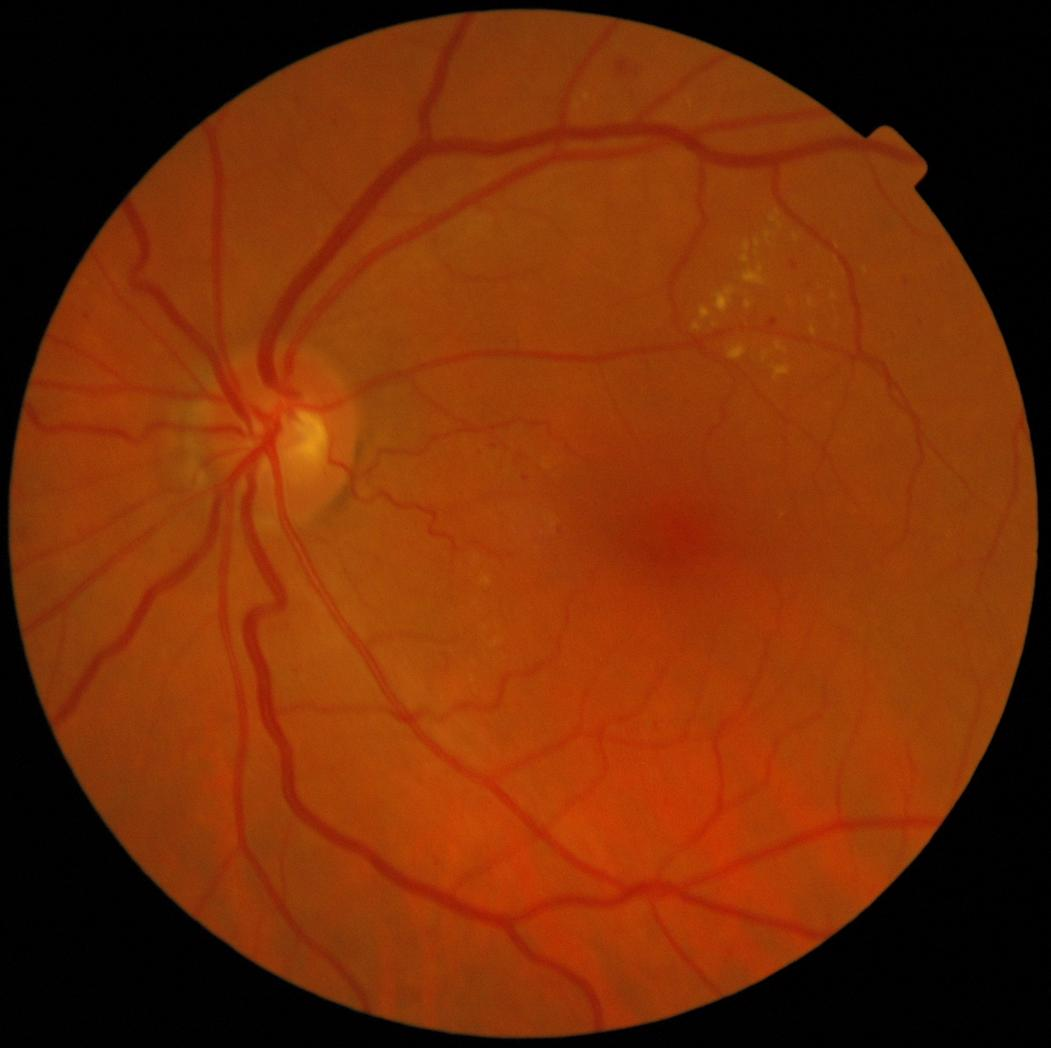
\includegraphics[width=50mm]{./Figures/cap4/vasos/vaso1.jpg}}
%\subfigure[Canal verde de la Imagen.]{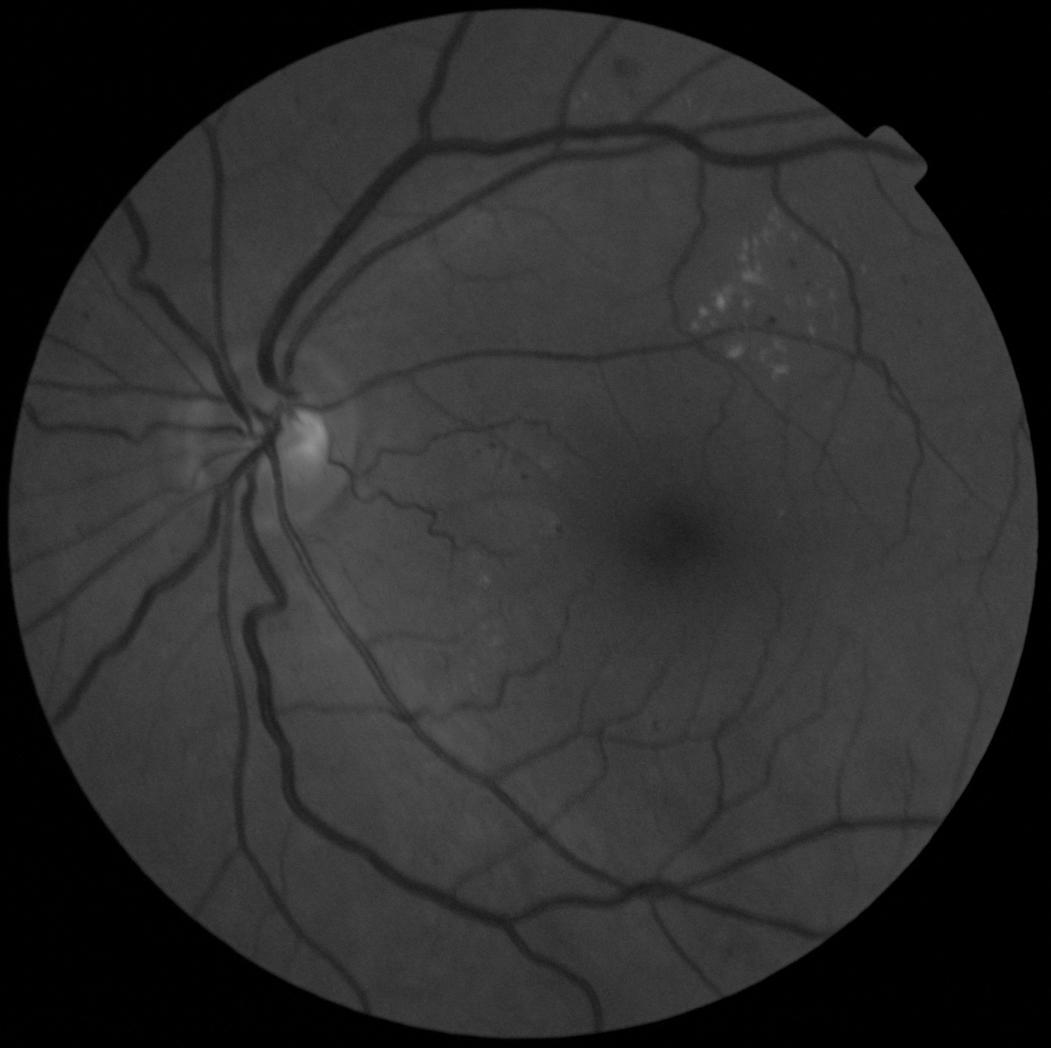
\includegraphics[width=50mm]{./Figures/cap4/micro0.jpg}}
%\caption{Canal verde de la imagen.} \label{fig:vaso_1}
%\end{figure}

%\subsubsection{CLAHE}
